\documentclass{article}
\usepackage[utf8]{inputenc}
\usepackage{amsmath}
\usepackage{graphicx}
\usepackage{textcomp}
\usepackage{enumerate}
\usepackage{float}
\usepackage{physics}


\title{
 Computational Physics Final Project \\ 
\begin{large} 
  Electrostatic Particle-In-Cell Method
\end{large} }
\author{Erica Kotta }
\date{December 16, 2016}

\begin{document}

\maketitle





\section{Intro to Particle-In-Cell Method}
A plasma is a gas whose atoms, due to certain conditions (high temperature, strong external EM fields, etc) have been ionized. Although the net charge of the plasma as a whole is generally zero, the constituent particles now carry a (positive or negative) charge. These charge-carrying particles now will interact not only with the external EM fields but will create their own fields, which will in turn affect their dynamics as well. 
\newline
To completely and accurately describe plasma dynamics entails calculating the force $F = q\left[\vec{E} + (\vec{v}\times\vec{B})\right]$ \textit{between each and every pair of particles}. This would mean, for a simulation of $N$ particles, $N^2$ calculations for one time step. Even in a very simplified model of a million particles, the simulation becomes quite impossible. 

Now, however, consider one particle--say, an electron, in this sea of particles in the plasma. It will attract positive ions (let's just say they are simple protons, for simplicity) and repel other electrons. The charge of this electron becomes effectively shielded by the surrounding protons, and the force felt by other particles in the area falls exponentially at a distance called the Debye length, defined by 

\begin{equation}
\lambda_{De} = \sqrt{\dfrac{\epsilon_0 k_B T_e}{q^2 n_0}}
\end{equation}

where $\epsilon_0$ is the permittivity of a vacuum, $k_B$ is the Boltzmann constant, $T_e$ the electron temperature, and $n_0$ is the plasma (electron) density. \newline
When we are working with spatial scales larger than the Debye length, the dynamics are not dominated by the interactions of closest neighboring pairs, and we start to see the collective behavior of particles. 
\newline
\indent Furthermore, if we consider spatial scales larger than $\lambda_{De}$ we can also use the concept of \textit{superparticles}, which is simply a clump of many (usually around the ballpark of $10^6$) individual particles. A superparticle will behave similarly to an individual particle. \newline
\newline
\newline 
\indent Equipped with these simplifications, we start to see that plasma simulation can in fact be modelled. Here I introduce the Particle-In-Cell (PIC) method. It uses the concept of superparticles along with the neat trick of approximating their charges and thus EM fields at the points of a grid, and using these grid EM values to move the particles one step at a time. Below I describe the basic structure of the PIC code I wrote for a simple 2-D plasma in the electrostatic case (ignoring all B-fields).\newline \newline
\textbf{Disclaimer:} I should warn that this is a \textit{very} qualitative and simplified program; I use toy negative superparticles of total charge -1.0 and mass 0.1, and positive superparticles of total charge +1.0 and mass 1.0. Epsilon is also set to 1.0. This code is light years away from being a tool for studying plasma physics, and instead is simply a demonstration of the basics of the PIC method. Qualitative, unitless graphs in the final section simply show that the code is not overwhelmed by non-physics. \newline
\newline


\section{Interpolating Particle Charges to the Grid}
Let's look at a (2-D) portion of the plasma. We section each dimension into N slices (Nx, Ny), each slice ($\Delta x, \Delta y$) set to ~$\lambda_{De}$ (this ensures we are working at an appropriate scale). Now rather than keeping track of the individual superparticle positions, we weigh the charge to the four grid points surrounding it according to the figure: 
\begin{figure}[H]
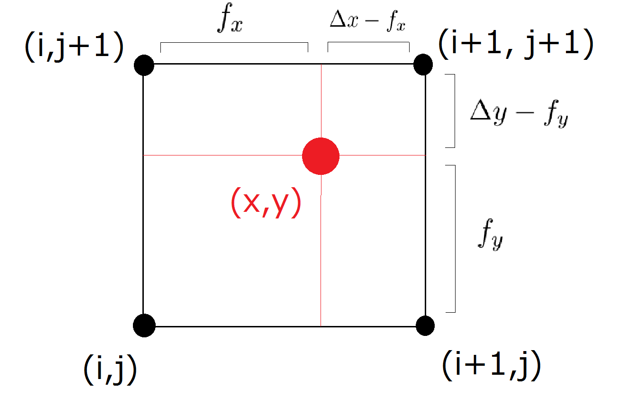
\includegraphics[scale=0.7]{weigh.png}
\centering
\end{figure}
Grid point (i,j) gets assigned charge proportional to $\dfrac{(\Delta x - f_x)\times(\Delta y - f_y)}{\Delta x \Delta y}$, point (i+1,j) gets $\dfrac{(\Delta x - f_x)\times(f_y)}{\Delta x \Delta y}$, etc. We do this for all grid points, with the boundary and corner points getting doubled overall (as the area contributing to these points is a half of the others; corner points get doubled twice). \newline
\newline 


\section{Using FFT to calculate scalar potential V}
With the charges distributed to the grid, we can now approximate the scalar potential field at the grid points from the relationship:
\begin{equation}
\dfrac{\partial^2V_{ij}}{\partial x^2} + \dfrac{\partial^2V_{ij}}{\partial y^2} = -\dfrac{1}{\epsilon_0}\rho_{ij}
\end{equation}
which can be discretized to 
\begin{equation}
\dfrac{(V_{i+1, j} + V_{i-1,j} - 4V_{i,j} + V_{i,j+1} + V_{i,j-1})}{\Delta x\Delta y} = -\dfrac{1}{\epsilon_0}\rho_{ij}
\end{equation}
We can solve for $\phi$ using the Jacobian method as outlined in the course textbook using the 5-point stencil. If however we can assume periodicity in both directions (which we can in our case, if we are looking at a small chunk in the middle of a huge cloud of plasma), it is we can use the Fourier method, which is much faster. The 2-D FT of $V_{ij}$ and $\rho_{ij}$ are (using $i^*$ to indicate $\sqrt{-1}$ differently from index $i$ and setting $N_x=N_y=N$):
\begin{equation}
\begin{split}
V_{mn} &= \dfrac{1}{N}\sum_{i=0}^{N-1}\sum_{j=0}^{N -1}\exp{\dfrac{2i^*\pi(mi + nj)}{N}}V_{ij} \\
\rho_{mn} &= \dfrac{1}{N}\sum_{i=0}^{N-1}\sum_{j=0}^{N-1}\exp{\dfrac{2i^*\pi(mi +nj)}{N}}\rho_{ij}
\end{split}
\end{equation}
which inverse-transform to
\begin{equation}
\begin{split}
V_{ij} &= \dfrac{1}{N}\sum_{m=0}^{N-1}\sum_{n=0}^{N-1}\exp{\dfrac{2i^*\pi(-im-jn)}{N}}V_{mn}\\
\rho_{ij} &= \dfrac{1}{N}\sum_{m=0}^{N-1}\sum_{n=0}^{N-1}\exp{\dfrac{2i^*\pi(-im-jn)}{N}}\rho_{mn}
\end{split}
\end{equation}
Plugging the FT expressions of $V_{ij}$ and $\rho_{ij}$ into the discretized equation, dividing both sides by $\dfrac{1}{N}e^{2i^*\pi(-im-jn)/N}$ and looking at one (m,n) point at a time (so taking out the $\sum$'s), we get 
\begin{equation}
V_{mn} = \dfrac{\rho_{mn}(\Delta x\Delta y)}{\exp{\dfrac{-2i\pi m}{N}}+\exp{\dfrac{2i\pi m}{N}}-4+\exp{\dfrac{-2i\pi n}{N}}+\exp{\dfrac{2i\pi n}{N}}}
\end{equation}
and inverse-FT-ing these $V_{mn}$ values gives us back $V_{ij}$. \footnote{Note that due to Python's default indexing of arrays versus plot points, a specified x-value from plot (x,y) will correspond to the j-value of grid point (i,j), and vice versa.} These steps are implemented in the code using numpy's rfft2 and irfft2 functions. 

\section{Calculating E-field}
Using the newly calculated values $V_{ij}$, we can now calculate the electric field. Its true definition is the (negative) gradient of the potential; in the code we approximate this with finite differencing (central method), finding the Ex-field and Ey-field separately:
\begin{equation}
\begin{split}
E_{x,ij} &= -\dfrac{V_{i,j+1} - V_{i,j-1}}{2\Delta x}\\
E_{y,ij} &= -\dfrac{V_{i+1,j} - V_{i-1,j}}{2\Delta y}.
\end{split}
\end{equation}
and at the boundaries include lines in the code to use forward/backward differencing divided by ($1\times\Delta x,y$) to account for the lack of point on the other side.
\newline
Then we interpolate the field at the \textit{grid points} back onto the \textit{particles}. This is done in the exact same way as interpolating the particle charge onto the grid. In my code function for weighing the particles onto the grid, I stored and returned the (i,j) points and the corresponding weights, so just call these back in the function for this step. 

Below is an example plot showing the charge density (plotted using imshow), the calculated potential (the contour lines), and the resulting E-field (the quiver plot). 

\begin{figure}[H]
\begin{center}
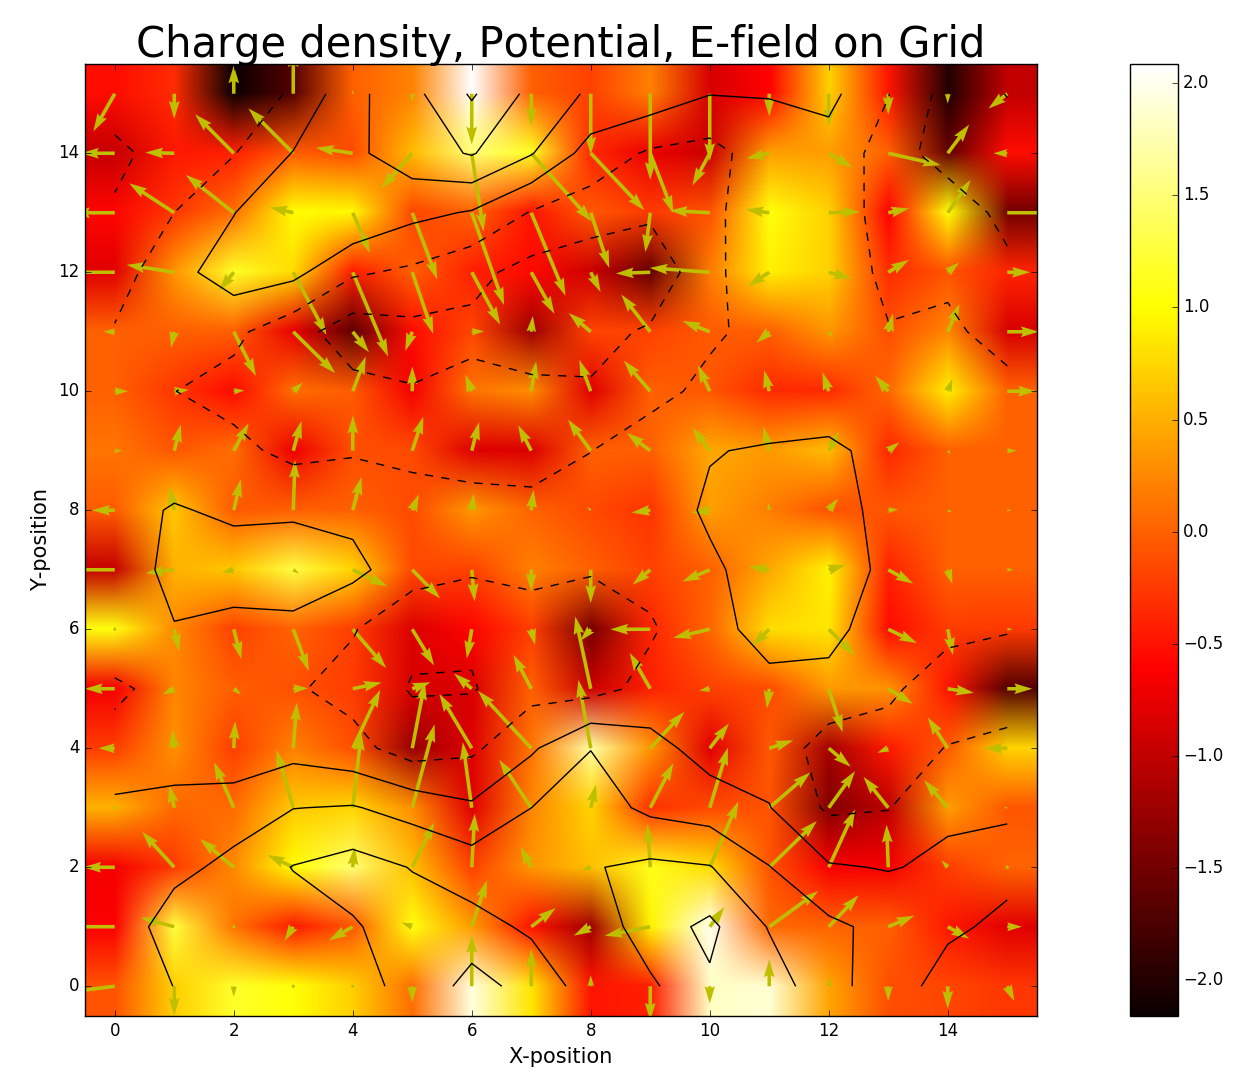
\includegraphics[scale=0.4]{nother_grid.png}
\caption{Density plot = Charge distribution; Contour lines = Scalar potential; Vector field = E-field}
\end{center}
\end{figure}

Though this is a very qualitative plot (see disclaimer at end of Section 1), you can see that the results make sense: the potential lines follow the charge grid as expected, with the calculated E-field vector field pointing in the correct directions and relative magnitudes along the potential gradient. 

\section{Advancing the Particles}
Now we have the strength of the electric field in the x- and y-direction for each particle in our section of the plasma, and will use the Leap-Frog method to advance each particle by one $\Delta t$ at a time. I chose this method because it is (supposedly) energy-conserving. \newline
The Courant-Friedrichs-Lewy condition for numerical stability in two dimensions is given by the formula 
\begin{equation}
\Delta t \leq \dfrac{CFL}{v_{x,max}/\Delta x + v_{y,max}/\Delta y}
\end{equation}
where $CFL$ is a constant less than 1. For plasmas, an equivalent condition is given by $\Delta t \leq \dfrac{0.2}{\omega_p}$ where $\omega_p$ is given by $\dfrac{q}{m}E_{max}$ and is the maximum $\Delta v$ for a given step. I only consider the values corresponding to the electrons here; their smaller relative mass means that they respond the most quickly to the fields, and thus impose the greatest restrictions on the time step. \newline \newline
The particles are advanced in the code in the simplest way: 
\begin{equation}
\begin{split}
\vec{v}_{new} &= \vec{v}_{old} + \Delta t\Big(\dfrac{q\vec{E}}{m}\Big) \\
\vec{x}_{new} &= \vec{x}_{old} + \Delta t(\vec{v}_{new})
\end{split}
\end{equation}
where $\vec{v}_{old}$ and $\vec{v}_{new}$ are the velocities at $t-\dfrac{\Delta t}{2}$ and $t + \dfrac{\Delta t}{2}$, and $\vec{x}_{old}$ and $\vec{x}_{new}$ are the positions at $t$ and $t + \Delta t$, respectively. At $t=0$ only, the initial velocity vector is decelerated by half a time step to set up the stagger. (The velocities are also accelerated by half a time step for each loop to un-stagger the positions and velocities for use in calculations of energy, etc.) 

\newline
One way to check, at least qualitatively, that the simulated dynamics are not completely non-physical is to plot the velocity distribution of the particles at certain times and check that they have a Maxwellian shape. \newline
Starting with particles distributed randomly throughout the area and with zero velocity, I plotted a histogram of the velocity distribution (in x-direction) at different times. The distribution almost immediately formed the Maxwellian shape, and maintained the shape for all consecutive steps. 
\begin{figure}[H]
\begin{center}
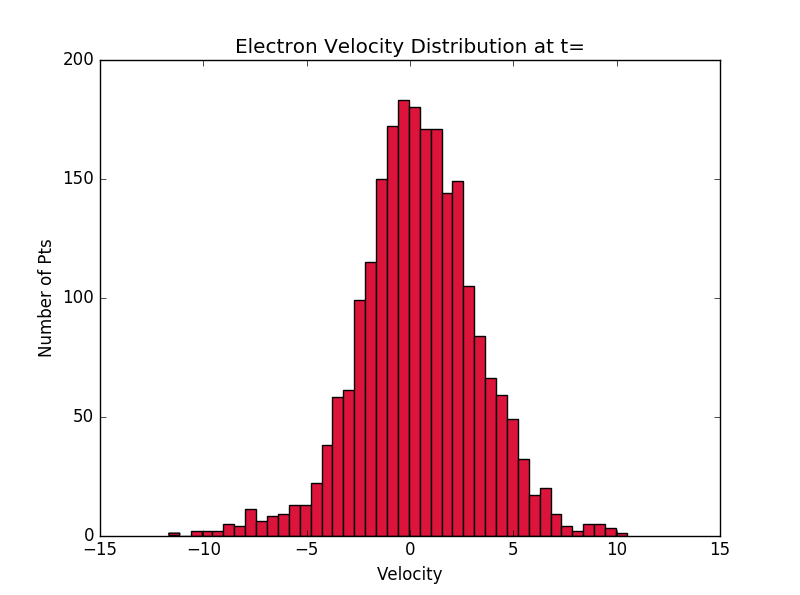
\includegraphics[scale=0.5]{vx_vel_dist.png}
\caption{Maxwellian shape apparent by first time iteration, maintains shape for all t.}
\end{center}
\end{figure}
Another sanity check is to plot a density plot of the position vs velocity. During equilibrium, the plot should be centered around v=0 and uniformly distributed position-wise. 
\begin{figure}[H]
\begin{center}
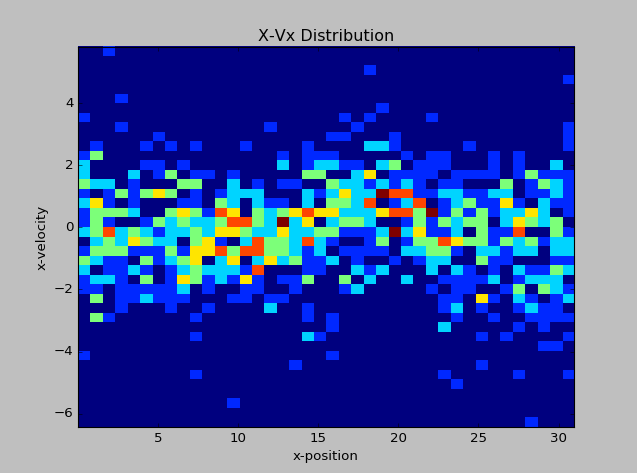
\includegraphics[scale=0.8]{X-vs_Vx_dist_imshow.png}
\caption{Particle velocities centered around v=0, distributed evenly in position.}
\end{center}
\end{figure}

Lastly, a plot of energy vs time shows how the code conserves energy. Though the graph shows that total energy is not precisely conserved and seems to gradually increase over time, there at least is an apparent anti-correlation between the kinetic and potential energy. 
\begin{figure}[H]
\begin{center}
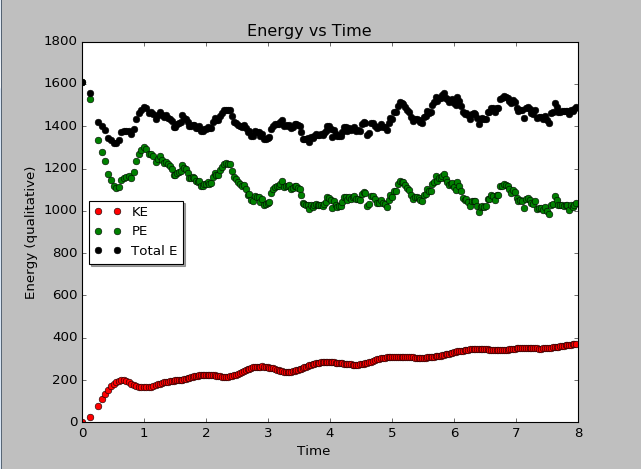
\includegraphics[scale=0.8]{E_vs_t_NxNy31Npt1000.png}
\end{center}
\end{figure}


\subsection{References}
\begin{thebibliography}{9}
\bibitem{PIC bible} 
C K Birdsall & A B Langdon. 
\textit{Plasma Physics Via Computer Simulation}. 
Adam Hilger, 1991.
 
\bibitem{other book} 
James J Y Hsu. 
\textit{Visual and Computational Plasma Physics}. 
World Scientific Publishing, 2015.
 
\bibitem{PIC website} 
The Electrostatic Particle In Cell (ES-PIC) Method
\\\texttt{https://www.particleincell.com/2010/es-pic-method/}
\end{thebibliography}





\end{document}

